\documentclass[submit,techreq,noauthor]{ipsj}

\usepackage[dvips]{graphicx}
%\usepackage{latexsym}

\usepackage{ascmac}
\usepackage{fancybox}
 
\newenvironment{cmd}
{
\VerbatimEnvironment
\begin{screen}
\scriptsize
\def\baselinestretch{.75}
\begin{Verbatim}
}
{
\end{Verbatim}
\end{screen}
}

\setcounter{巻数}{54}%vol54=2013
\setcounter{号数}{10}
\setcounter{page}{1}

% remove page number
%\pagestyle{empty}
%\parindent 0.5zw %% for English
%\parindent 1zw
% insert indent in head of section
\usepackage{indentfirst}

\begin{document}

\title{C++ をベースとする新しいハードウェア記述の検討}

%\etitle{}

\affiliate{TITECH}{東京工業大学 大学院情報理工学研究科}

\author{佐藤 真平}{Shimpei Sato}{TITECH}[satos@arch.cs.titech.ac.jp]
\author{吉瀬 謙二}{Kenji Kise}{TITECH}[kise@cs.titech.ac.jp]


\begin{abstract}
本稿では,RTL モデリングのための新しい言語として ArchHDL を提案する.
ハードウェアのレジスタを変数,ワイヤを関数として扱うことで,C++ で RTL モデリングを実現する.
ワイヤは,C++11 で定義されたラムダ関数を用いて記述する.
ArchHDL によるハードウェアの記述は Verilog HDL に近い.
ArchHDL を用いて記述したハードウェアは C++ のプログラムとしてコンパイル可能である.
また,論理シミュレーションを高速に行うことができる.
\end{abstract}

%\begin{jkeyword}
%\end{jkeyword}

%\begin{eabstract}
%\end{eabstract}

%\begin{ekeyword}
%\end{ekeyword}

\maketitle

\section{はじめに}

プロセッサなどのハードウェア設計は,アーキテクチャ設計,論理設計,回路設計,物理設計といったフローで行われる\cite{ito:2011}.
アーキテクチャ設計と論理設計においては,RTL(Register Transfer Level)のシミュレーションが不可欠である.
このために Verilog HDL などのハードウェア記述言語が用いられることが一般的である.


%既存のプログラミング言語を利用して実装された RTL モデリングを行うことができる言語として
%SystemC,MyHDL が挙げられる.


%抽象度の高いレベルで記述されるソフトウェアシミュレータでは,
%ハードウェアを意識した記述がなされることがある.
%設計するハードウェア規模が大きくなると,
%モジュールの呼び出しタイミングなどに制約が発生し,
%可読性や保守性の妨げとなる.
%例えば,パイプライン処理におけるフォワーディングを実装しようとする場合,
%パイプラインステージごとにモジュール化されているとすると,
%先行ステージを先に呼び出し,結果を後続のステージで使用するといった呼び出し順序の制約が発生する.

%論理設計の段階においては,Verilog HDL などのハードウェア記述言語を用いた論理検証が行われる.
%抽象度の高いレベルで記述されたソフトウェアシミュレータでおきる制約は
%ハードウェア記述言語による記述では発生しない.
%しかし,ハードウェア記述言語による論理シミュレーションは速度が遅く,
%パラメタ設定などの柔軟性に欠く.

本稿では,RTL の高速なシミュレーションを実現する \textbf{ArchHDL} を提案する.
ArchHDL は,ハードウェアの RTL モデリングのための新しい言語である.
ArchHDL は,ハードウェアの RTL モデリングを Verilog HDL に近い記述で行う.
この言語を用いることで,ハードウェアの論理検証を高速に行うことができる.

構成は以下の通りである.
2 章で,提案する ArchHDL を理解するために不可欠な C++11 のラムダ関数について述べる.
3 章で,ArchHDL を提案する.
4 章で,ArchHDL の予備評価を行い,5 章でまとめる.

\section{C++ のラムダ関数と使い方}
C++11 と呼ばれる C++ ISO 標準により,ラムダ関数の仕様が定義された.
GCC では,バージョン 4.5 よりこの ISO 標準の一部がサポートされ,
標準ライブラリとしてラムダ関数が利用できるようになった.

我々の提案する ArchHDL では,このラムダ関数を利用する.
ここでは,C++11 のラムダ関数の機能を ArchHDL のために必要な範囲で述べる.

\begin{figure}[t]
\begin{cmd}
1 int main() {
2   [=](int x, int y){ return x + y; };
3   return 0;
4 }
\end{cmd}
\caption{ラムダ関数の定義のみを含む C++ プログラムの例}
\label{src:lambda1}
\end{figure}

\figref{src:lambda1}にラムダ関数の定義のみを含む C++ プログラムの例を示す.
2 行目のコードは引数に int x と int y をとり,その和を返すラムダ関数の定義である.

ラムダ関数の定義は lambda-introducer と呼ばれる [] \footnote{
[] 内にキャプチャと呼ばれるラムダ関数の機能を指定する記述をする必要がある.
ArchHDL では [=] のみを使用するため説明は省略する.
}
の記述からはじまる.
ラムダ関数の返り値の型は,return 文より推測できる場合に省略できる.
例に示したラムダ関数の返り値の型は int と推測される.

%lambda-introducer について述べる.
%ラムダ関数は,それが定義されているスコープ内の変数を使用することができる.
%これを変数のキャプチャと呼び,lambda-introducer の [] の中にキャプチャ方法を記述する.
%\figref{src:lambda1}の例では,[]内になにも記述しておらず,スコープ内の変数のキャプチャは行わない.
%変数をキャプチャする場合は,コピーによるキャプチャと参照によるキャプチャの 2 種類がある.
%ラムダ関数が定義されているスコープ内に変数 a,b,c が定義されているとき,
%キャプチャは次のように記述する.
%\begin{itemize}
% \item \textbf{[]}:変数をキャプチャしない
% \item \textbf{[=]}:すべてコピーによるキャプチャ
% \item \textbf{[\&]}:すべて参照によるキャプチャ
% \item \textbf{[a, \&b]}:a はコピー,b は参照によるキャプチャ
% \item \textbf{[=, \&a]}:a のみ参照,他はコピーによるキャプチャ
% \item \textbf{[\&, a]}:a のみコピー,他は参照によるキャプチャ
%\end{itemize}
%コピーによるキャプチャは,ラムダ関数外の変数の値をコピーしてラムダ関数内で使用する.
%参照によるキャプチャは,ラムダ関数外の変数の参照をラムダ関数内で保持する.
%ラムダ関数をあるクラスのメンバ関数内で定義したときに,
%そのメンバ変数をキャプチャする場合は参照によるキャプチャのみとなる.
%ArchHDL ではコピーによるキャプチャのみを利用するため [=] という記述のみ使用するが,
%メンバ変数をキャプチャする場合があり,このときは暗黙に参照によるキャプチャとなっている.
 
\begin{figure}[t]
\begin{cmd}
 1 #include <functional>
 2
 3 int main() {
 4   int a = 2;
 5   int b = 3;
 6   std::function<int ()> Sum =
 7                     [=](int x, int y) { return x + y; };
 8   int c = Sum(a, b);
 9   return 0;
10 }
\end{cmd}
\caption{ラムダ関数を定義して,それを使う C++ プログラムの例}
\label{src:lambda2}
\end{figure}

\figref{src:lambda2} にラムダ関数を定義して,それを使う C++ のプログラムを示す.
ラムダ関数を使うために,1 行目のように functional という標準ライブラリをインクルードする.

6,7 行目で, 関数オブジェクト Sum に [=](int x, int y) \{ return x + y; \} というラムダ関数を代入する.
このラムダ関数は int 型の値を返す関数であり,その型は std::function$<$int ()$>$ となる.
これにより,Sum は 2 個の int 型の値を引数にとり,その和を返す関数オブジェクトとなる.

8 行目では Sum を呼び出し,返り値を変数 c に代入している.
引数には,4, 5 行目にある a, b を与えている.

ArchHDL では,ラムダ関数を\figref{src:lambda2}のような使い方をしている.

\section{ArchHDLの提案}

ArchHDL はハードウェアの RTL モデリングのための言語である.
Verilog HDL に近い記述方法を目指している.
ユーザはライブラリにより提供される Module クラス,reg クラス,wire クラスおよび C++11 のラムダ関数を用いて
ハードウェアを記述する.

\subsection{ArchHDL の制約}
ArchHDL には,次に挙げる制約がある.
\begin{itemize}
 \item 単一クロックの立ち上がりエッジのみでレジスタの値を更新
 \item 32 ビットや 64 ビットなどの整数型をベースとした記述
\end{itemize}

実装を簡潔にするために単一クロックの同期回路で,
かつレジスタへの代入はクロックの立ち上がりエッジのみのハードウェアを対象とする.
複数のクロックや,クロックの立ち上がりエッジと立ち下がりエッジでの制御はサポートしていない.

演算に用いるデータ型として,C++ 言語の32 ビットや 64 ビットなどの整数型を使用する.
任意のビット幅のレジスタやワイヤはサポートしていない.
演算子は C++ が提供する演算子をサポートしており,
Verilog HDL で使用可能なビット切り出しやビット連結などの演算はサポートしない.

\subsection{ArchHDL の利点}
ArchHDL には,次に挙げる利点がある.
\begin{itemize}
 \item ハードウェアモジュール間の接続の記述が容易
 \item 論理シミュレーションが高速
\end{itemize}
ここでは特に重要な前者について述べる.

\begin{figure}[t]
 \begin{center}
  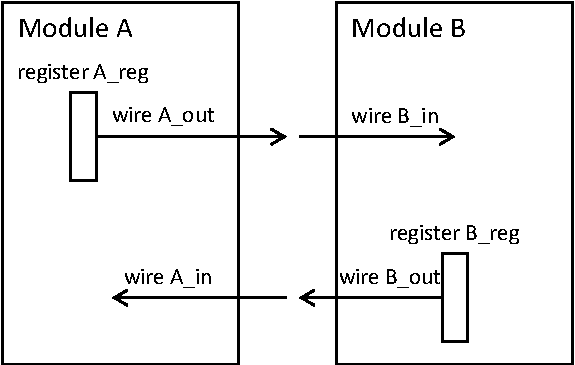
\includegraphics[width=.4\textwidth,keepaspectratio,clip]{fig/module.eps}
  \caption{手続き型言語では記述が難しいモジュール間の接続の例}
  \label{fig:module}
 \end{center}
\end{figure}

\figref{fig:module} に,手続き型言語でハードウェアの挙動を記述しようとすると,
記述が難しいモジュール間の接続の例を示す.
モジュール A は入力ワイヤ A\_in,出力ワイヤ A\_out の入出力を持つ.
出力ワイヤ A\_out はレジスタ A\_reg の値を出力する.
モジュール B は入力ワイヤ B\_in,出力ワイヤ B\_out の入出力を持つ.
出力ワイヤ B\_out はレジスタ B\_reg の値を出力する.

モジュール A の出力ワイヤ A\_out は モジュール B の入力ワイヤ B\_in に接続している.
モジュール B の出力ワイヤ B\_out は モジュール A の入力ワイヤ A\_in に接続している.
モジュール A は,あるサイクルに入力として B\_reg の値を受け,A\_reg の値を出力するというモジュールである.
同様に,モジュール B は,あるサイクルに入力として A\_reg の値を受け,B\_reg の値を出力するというモジュールである.

\begin{figure}[t]
 \begin{center}
  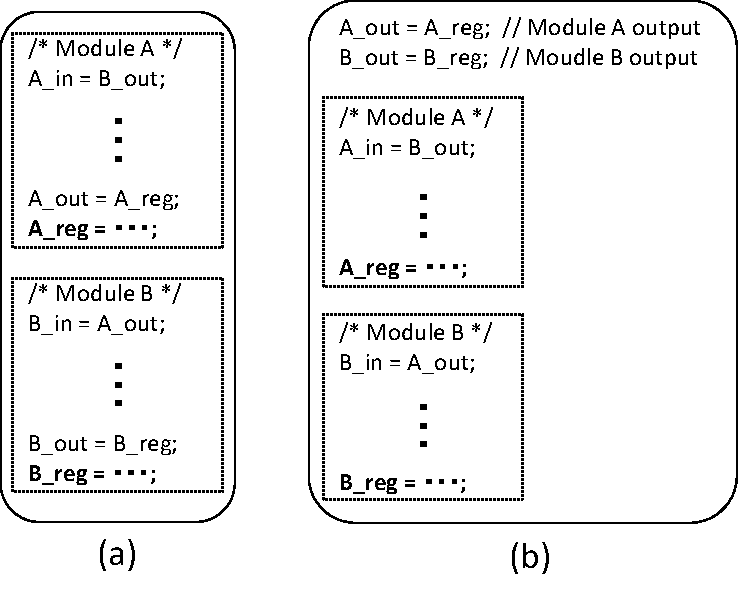
\includegraphics[width=.4\textwidth,keepaspectratio,clip]{fig/module2.eps}
  \caption{\figref{fig:module}のハードウェアの記述例}
  \label{fig:module2}
 \end{center}
\end{figure}

このハードウェアの挙動をモジュールごとに記述すると,\figref{fig:module2}(a)のようになる.
この記述は,
モジュールへの入力,モジュール内の処理,モジュールからの出力,レジスタの更新という
まとまりのある記述になっている.
レジスタの更新は図中の太字で示した箇所である.

手続き型言語で
\figref{fig:module2}(a)のように順番にモジュール A,モジュール B の処理が記述される場合,
モジュール A の処理の先頭にある A\_in への代入は,1 サイクル前の B\_out の状態となり,
\figref{fig:module}のハードウェアとは異なる挙動となる.

このハードウェアの挙動を手続き型言語で記述するには,
\figref{fig:module2}(b)のようにレジスタからの読み出しをモジュールごとの処理とは別に
記述するといった対策が必要である.
しかし,このような記述はモジュールが複雑になればなるほど呼び出し順序に依存関係が生じ,
保守性や可読性が損なわれる.

Verilog HDL などのハードウェア記述言語では継続代入やノン・ブロッキング代入のサポートにより
呼び出し順序に依らないハードウェアの記述が可能である.
ArchHDL では,ライブラリにより提供されるクラス群を使用してハードウェアを記述すれば,
先に例示したようなモジュールの接続も Verilog HDL 同様に記述することができる.

\subsection{ArchHDL による RTL モデリング}
ArchHDL を用いた RTL モデリングでは,
ライブラリにより提供される Module クラス,reg クラス,wire クラスおよび,C++11 のラムダ関数を用いて
ハードウェアを記述する.

\begin{figure}[t]
\begin{cmd}
 1 class Counter : public Module {
 2  public:
 3   wire<uint> out;
 4   reg<uint> counter;
 5   void Init() {
 6     out = [=]() { return counter(); };
 7   }
 8   void Always() {
 9     counter <<= (counter() + 1) & 0xff;
10   }
11 };
\end{cmd}
\caption{ArchHDL による 8 ビットカウンタ回路の記述}
\label{src:counter}
\end{figure}

\begin{figure}[t]
\begin{cmd}
 1 module Counter(CLK, out);
 2     input CLK;
 3     output [7:0] out;
 4
 5     reg [7:0] counter;
 6     assign out = counter;
 7     always @(posedge CLK) begin
 8         counter <= counter + 1;
 9     end
10 endmodule
\end{cmd}
\caption{Verilog HDL による 8 ビットカウンタ回路の記述}
\label{src:counter_v}
\end{figure}

\figref{src:counter}に,ArchHDL を用いて記述した 8 ビットカウンタ回路のコードを示す.
また,\figref{src:counter_v} に,Verilong HDL で記述した 8 ビットカウンタ回路のコードを示す.
ArchHDL において,Module クラスを継承して定義されるクラス(Module 子クラス)は,
Verilog HDL におけるモジュールに相当する.
同様に reg クラス,wire クラスは,それぞれ Verilog HDL におけるレジスタ,ワイヤに相当する.

Module 子クラスは,そのメンバ関数として Init 関数および Always 関数を定義する必要がある.
これは,ライブラリにより強制されており,いずれかの関数が必要でない場合でも空の関数を定義する必要がある.

Init 関数には,モジュール内のすべてのワイヤへの継続代入の定義を記述する.
これは,Verilog HDL においてモジュール内で定義されている assign 文をすべてこの関数内に記述することに相当する.
wire クラスのインスタンスにラムダ関数を代入することでワイヤへの継続代入を記述することができる.
\figref{src:counter}では,6 行目で wire クラスの変数 out に reg クラス の counter の値を返す
ラムダ関数([=]() { return counter(); })を代入している.
ここで,reg クラスのオブジェクトは関数として呼び出すことにより,そのサイクルにおける値を取得することができる.
このため,先のラムダ関数における counter() によってレジスタの値が取得できる.
これは,\figref{src:counter_v} の 6 行目に相当する.

Always 関数には,モジュール内のすべてのレジスタへのノン・ブロッキング代入を記述する.
ArchHDL では,単一クロックの立ち上がりエッジでの制御のみを対象としている.
これは,Verilog HDL における '' always @(posedge clock)`` ブロック内の記述に相当する.
reg クラスのインスタンスに$<<=$演算子を用いて値を代入することでノン・ブロッキング代入を記述することができる.
ArchHDL は,演算子オーバーロードを利用して$<<=$演算子を Verilog HDL における
ノン・ブロッキング代入に相当する値の代入として実装している.
\figref{src:counter}では,9 行目で reg クラスの変数 counter に自身の値をインクリメントした値を代入している.
これは,\figref{src:counter_v}の 8 行目に相当する.

ArchHDL では,データ型として C++ の整数型を使用している.
\figref{src:counter}の例では unsigned int 型を利用しているため,
8 ビットカウンタを実現するために値をマスクする必要がある.
reg クラスと wire クラスのオブジェクトは関数として呼び出すことにより,そのサイクルにおける値を取得することができる.

\subsection{テストベンチの記述}
ArchHDL は,C++ 言語をベースとしている.
したがって,ユーザは柔軟にテストベンチを記述することが可能である.
ここでは,ArchHDL の提供するライブラリを用いたテストベンチ記述の一例を示す.

\begin{figure}[t]
\begin{cmd}
 1 class TestTop : public Module {
 2  public:
 3   reg<uint> HALT;
 4   reg<uint> cycle;
 5 
 6   wire<uint> cnt_out;
 7   Counter cnt;
 8    
 9   void Init() {
10     cnt_out = cnt.out;
11   }
12   void Always() {
13     cycle <<= cycle() + 1;
14     HALT  <<= (cycle() >= HALT_CYCLE);
15
16     if (cycle() > (HALT_CYCLE - 10)) {
17       printf("%d %u\n", cycle(), cnt_out());
18     }
19   }
20 };
21
22 int main() {
23   TestTop testtop;
24   while (!testtop.HALT()) {
25     ArchHDL::Step();
26   }
27   return 0;
28 }
\end{cmd}
\caption{ArchHDL を用いたカウンタ回路のためのテストベンチの記述例}
\label{src:test}
\end{figure}

\figref{src:test} は,先に示したカウンタ回路の ArchHDL によるテストベンチの記述例である.
インクルードの記述などは省略している.また,14 行目と 16行目の HALT\_CYCLE は定数である.

このテストベンチ記述は,テストモジュール TestTop を作成し,
その中でカウンタ回路のインスタンスを生成しテストを行うという設計になっている.
そのために,22 行目からの main 関数は簡潔になり,TestTop モジュールのインスタンス生成と
ライブラリによりステップ実行のみの記述となる.

ArchHDL は,モジュールのインスタンスを生成する際にすべての reg クラスのインスタンス,
wire クラスのインスタンスをライブラリで一元管理する設計になっている.
そのため,23 行目のようにモジュールのインスタンスを生成したのち,
ArchHDL により提供される Step 関数(25行目)を呼び出せばサイクルごとのシミュレーションができる.

\begin{figure}[t]
\begin{cmd}
 1 module TestTop();
 2     reg CLK;
 3     reg  [31:0] cycle;
 4 
 5     wire [7:0] ot_cnt;
 6     Counter cnt(CLK, ot_cnt);
 7
 8     initial begin
 9         CLK = 0;
10         cycle = 0;
11         cnt.cnt = 0;
12     end
13 
14     always #50 CLK = ~CLK;
15 
16     always @(posedge CLK) begin
17         cycle <= cycle + 1;
18         if (cycle > (`HALT_CYCLE - 10))
19             $write("%d %d\n", cycle, ot_cnt);
20         if (cycle >= `HALT_CYCLE) $finish;
21     end
22 endmodule
\end{cmd}
\caption{Verilog HDL を用いたカウンタ回路のためのテストベンチの記述例}
\label{src:test_v}
\end{figure}

\figref{src:test} に挙げたテストベンチの記述は,Verilog HDL で同様の記述ができるという利点がある.
\figref{src:test_v} に Verilog HDL を用いて同様のテストベンチを記述する例を示す.
ArchHDL を用いた場合と大きく異なる点は 14 行目においてクロックを生成している部分である.
それ以外の記述については ArchHDL と Verilog HDL で大きな違いはない.

\subsection{ArchHDL の実装}
\subsubsection{ソフトウェアアーキテクチャ}
ArchHDL のライブラリには,Module クラス,wire クラス,reg クラス,これらの 3 個のクラスのインタフェースクラス,
Singleton クラスの 7 個のクラスが定義されている.
本章では,標準ライブラリのインクルードをのぞくすべてのライブラリのコードを示しながら ArchHDL の実装について述べる.
以降の説明では,ユーザが Module クラスを継承して作成したクラスを Module 子クラスと呼ぶ.

\begin{figure}[t]
\begin{cmd}
 1 class RegisterInterface {
 2  public:
 3   virtual void Update() = 0;
 4 };
 5
 6 class ModuleInterface {
 7  public:
 8   virtual void Init() = 0;
 9   virtual void Always() = 0;
10 };
11
12 class WireInterface {};
13 
14 namespace ArchHDL {
15
16 class Singleton {
17  private:
18   std::vector<RegisterInterface*> registers_;
19   std::vector<ModuleInterface*> modules_;
20   std::vector<WireInterface*> wires_;
21  public:
22   static Singleton& GetInstance(void) {
23     static Singleton singleton;
24     return singleton;
25   }
26   void AddRegister(RegisterInterface* ri) {
27     registers_.push_back(ri);
28   }
29   void AddModule(ModuleInterface* mi) {
30     modules_.push_back(mi);
31   }
32   void AddWire(WireInterface* wi) {
33     wires_.push_back(wi);
34   }
35   void Init() {
36     for (uint i = 0; i < modules_.size(); i++) {
37       modules_[i]->Init();
38     }
39   }
40   void Exec() {
41     for (uint i = 0; i < modules_.size(); i++) {
42       modules_[i]->Always();
43     }
44     for (uint i = 0; i < registers_.size(); i++) {
45       registers_[i]->Update();
46     }
47   }
48 };
49
50 void Step() {
51   static bool init = false;
52   if (!init) {
53     init = true;
54     ArchHDL::Singleton::GetInstance().Init();
55   }
56   ArchHDL::Singleton::GetInstance().Exec();
57 }
58
59 }  // namespace ArchHDL
\end{cmd}
\caption{ArchHDL ライブラリにおける各インタフェースクラスと Singleton クラスと Step 関数の定義}
\label{src:class_singleton}
\end{figure}

\figref{src:class_singleton} に RegisterInterface クラス,ModuleInterface クラス,WireInterface クラス,
Singleton クラスおよび Step 関数の定義を示す.

ModuleInterface クラス,WireInterface クラス,RegisterInterface クラスは
それぞれ Module クラス,wire クラス,reg クラスのインタフェースクラスである.
Singleton クラスが,Module 子クラス,wire クラス,reg クラスのインスタンスを
シングルトン・パターンにより一元管理する.
これは,ArchHDL のライブラリにおいて核となるクラスである.

Singleton クラスは,メンバ変数として Module クラス,wire クラス,reg クラスの
インタフェースクラスのポインタを格納する可変行列をもつ(18 ~ 20 行目).
Module 子クラス,wire クラス,reg クラスのインスタンスが生成される際に,
そのインスタンスへのポインタが Singleton クラスに渡される.
また,ポインタは Singleton クラスに渡される際にそれぞれのインタフェースクラスに自動でアップキャストされる
(26 ~ 34 行目).

Step 関数(50 ~ 57 行目)は,1 サイクルのシミュレーションを行う関数である.
Step 関数を呼び出すと,Singleton クラスの Exec 関数が呼ばれる.
ただし,初回 Step 関数の呼び出しのみ Singleton クラスの Init 関数が呼ばれる.
Step 関数を繰り返し呼び出すことにより,複数サイクルにわたるシミュレーションが行なわれる.

Init 関数(35 ~ 39 行目)は,保持しているすべての Module 子クラスのインスタンスの Init 関数を呼ぶ(37 行目).
%これにより,ユーザが Module 子クラス内に定義したワイヤの継続代入の処理が行われる.

Exec 関数(40 ~ 47 行目)は,保持しているすべての Module 子クラスのインスタンスの Always 関数を呼び(42 行目),
次に保持しているすべての reg クラスのインスタンスの Update 関数を呼ぶ(45 行目).

Always 関数によりすべてのレジスタについて次のサイクルにおける値が計算される.
Update 関数によりレジスタの値が更新される.
この Always と Update の処理によりレジスタのノン・ブロッキング代入を実現する.


\subsubsection{reg クラスの定義}
\begin{figure}[t]
\begin{cmd}
 1 template <typename T>
 2 class reg : public RegisterInterface {
 3  private:
 4   bool set_;
 5   T curr_;
 6   T next_;
 7 
 8   // copy constructor
 9   reg<T>(const reg<T>& other);
10   reg<T>& operator=(const reg<T>& rhs);
11  public:
12   reg(): set_(false), curr_(0), next_(0) {
13     ArchHDL::Singleton::GetInstance().AddRegister(this);
14   }
15   void Update() {
16     if (set_) {
17       curr_ = next_;
18       set_ = false;
19     }
20   }
21   void operator=(T val) {
22     curr_ =  val;
23   }
24   void operator<<=(T val) {
25     set_ = true;
26     next_ = val;
27   }
28   T operator ()() {
29     return curr_;
30   }
31 };
\end{cmd}
\caption{ArchHDL ライブラリにおける reg クラスの定義}
\label{src:reg}
\end{figure}

\figref{src:reg} に,reg クラスの定義を示す.
reg クラスは,扱うデータ型をテンプレート引数にとるテンプレートクラスである.
また,インタフェースクラスである RegiterInterface クラスを継承する.

ArchHDL ではレジスタを変数として扱うため,
reg クラスはメンバ変数にテンプレート引数で与えられたデータ型の変数 curr\_ と next\_ を持つ(5,6 行目).
curr\_ は,あるサイクルにおけるレジスタの値で,next\_はその次のサイクルのレジスタの値である.
Module 子クラスの Always 関数の呼び出しにより,next\_に値が代入される.
reg クラスのメンバ関数 Update を呼ぶことで,next\_ の値は curr\_ に反映される(15 ~ 20 行目).
これによりレジスタへのノン・ブロッキング代入の挙動を実現する.

reg クラスのオブジェクトへの値の代入をそのメンバ変数 next\_ への値の代入とするために,
演算子オーバーロードにより $<<=$ 演算子を再定義している(24 ~ 27 行目).
$<<=$ 演算子により代入された値は,変数 next\_ に格納され,set\_ フラグがセットされる.

ArchHDL では,
すべての Module 子クラスのインスタンスの Always 関数を呼び出した後に,
すべての reg クラスのインスタンス Update 関数を呼び出す.
したがって,Always 関数が呼び出されている間に取得できる
レジスタの値 curr\_ は Update 関数が呼ばれるまで保持されている.

reg クラスのコンストラクタ(12 ~ 14 行目)では,
メンバ変数を初期化し,自身のポインタを Singleton クラスに渡す処理が行われる.
テスト記述や初期値設定のために = 演算子による値の代入も定義されている(21 ~ 23 行目).
= 演算子による値の代入は,式が評価された時点で curr\_ の値を変更する.
reg クラスのインスタンスを関数として呼び出すことで curr\_の値を取得することができる(28 ~ 29 行目).

\subsubsection{wire クラスの定義}
\begin{figure}[t]
\begin{cmd}
 1 template <typename T>
 2 class wire : public WireInterface {
 3  private:
 4   std::function<T ()> lambda_;
 5 
 6   // copy constructor
 7   wire<T>(const wire<T>& other);
 8   wire<T>& operator=(const wire<T>& rhs);
 9  public:
10   wire(): lambda_(nullptr) {
11     ArchHDL::Singleton::GetInstance().AddWire(this);
12   }
13   void operator=(std::function<T ()> lambda) {
14     lambda_ = lambda;
15   }
16   T operator()() {
17     return lambda_();
18   }
19 };
\end{cmd}
\caption{ArchHDL ライブラリにおける wire クラスの定義}
\label{src:wire}
\end{figure}

\figref{src:wire} に,wire クラスの定義を示す.
wire クラスは,テンプレート引数として扱うデータ型をとるテンプレートクラスである.
また,インタフェースクラスの WireInterface クラスを継承している.

ArchHDL では,ワイヤは関数として扱うため,
wire クラスはメンバ変数にラムダ関数 lambda\_ を持つ(4 行目)クラスとなっている.
このラムダ関数は,テンプレート引数として与えられたデータ型を返す関数である.

コピーコンストラクタの禁止(7,8 行目)と演算子のオーバーロード(13,14 行目)により,
wire クラスへの = 演算子による代入はラムダ関数に限定される.
これにより,wire クラスのオブジェクトは Module 子クラスの Init 関数で記述される
ラムダ関数を保持するクラスとなる.

wire クラスのコンストラクタ(10 ~ 12 行目)では,
メンバ変数を初期化し,自身のポインタを Singleton クラスに渡す処理が行われる.
wire クラスのオブジェクトを関数として呼び出すと,
自身の持つラムダ関数を呼び出した結果を返す(16 ~ 18 行目).
これにより,wire クラスのオブジェクトを関数呼び出しすることで,
そのサイクルでのワイヤの値が取得できる.

\subsubsection{Module クラスの定義}
\begin{figure}[t]
\begin{cmd}
 1 class Module : public ModuleInterface {
 2  private:
 3   // copy constructor
 4   Module(const Module& other);
 5   Module& operator=(const Module& rhs);
 6  public:
 7   Module() {
 8     ArchHDL::Singleton::GetInstance().AddModule(this);
 9   }
10   virtual void Init() {}
11   virtual void Always() {}
12 };
\end{cmd}
\caption{ArchHDL ライブラリにおける Module クラスの定義}
\label{src:module}
\end{figure}

\figref{src:module} に,Module クラスの定義を示す.
Module クラスは,インタフェースクラスの ModuleInterface クラスを継承するクラスである.
ArchHDL でハードウェアを記述する際に,このクラスを継承してモジュールを記述する.

コンストラクタ(7 ~ 9行目)では,自身のポインタを Singleton クラスに渡す.
ModuleInterface クラスにおいて Init 関数と Always 関数が仮想関数として定義されているため,
これらの関数を定義する必要がある.
Module クラスは,Module 子クラスのインタフェースとして定義しているため,
Init 関数と Always 関数として空の関数を定義している(10,11 行目).

\section{予備評価}
ArchHDL で記述したハードウェアのシミュレーション速度について
Verilog HDL で記述し Icarus Verilog\cite{iverilog} でコンパイルした場合と比較する.
本稿では,オープンソースの Verilog HDL コンパイラである Icarus Verilog を比較対象とする.

予備評価のために,
3 章で示した 8 ビットカウンタのインスタンスを 1024 個生成したハードウェアを使用する.
ArchHDL では,unsigned int 型のレジスタをマスクして 8 ビットのレジスタを実装している.
10 M サイクルのシミュレーション時間を time コマンドにより計測する.

シミュレーション環境は次の通りである.
\begin{itemize}
 \item CPU:Intel Core i7-3770K
 \item メモリ:32 GB
 \item OS:Ubuntu 12.04
 \item GCC:バージョン 4.6.3,最適化オプション -O3
 \item Icarus Verilog:バージョン 0.9.5
\end{itemize}

ArchHDL で記述したハードウェアを GCC でコンパイルした場合のシミュレーション時間は 42.9 秒である.
Verilog HDL で記述したハードウェアを Icarus Verilog でコンパイルした場合のシミュレーション時間は 2366 秒である.
このとき,ArchHDL の シミュレーション時間は,Verilog HDL に対して 55.2 倍の速度向上である.
予備評価の結果から,ArchHDL を用いたシミュレーションが大幅に速度向上することを確認した.

なお,予備評価のために用いたハードウェアは,ある程度の規模があるものの現実的とは言えない.
複雑で現実的なハードウェアを用いた評価は今後の課題である.

\section{まとめ}
ハードウェアの RTL モデリングのための新しい言語として ArchHDL を提案した.
ハードウェアのレジスタを変数,ワイヤを関数として扱うことで,C++ で RTL モデリングを実現する.
ワイヤは,C++11 で定義されたラムダ関数を用いて記述する.

ArchHDL によるハードウェア記述は, Verilog HDL に近い.
手続き型言語でハードウェアの挙動を記述しようとすると,
呼び出し順序に依存関係が生じ記述が難しい.
そのようなハードウェアの例を用いて,
ArchHDL が Verilog HDL のようにハードウェア記述ができることを述べた.

ArchHDL を用いて記述したハードウェアは C++ のプログラムとしてコンパイル可能である.
Verilog HDL で記述したハードウェアを Icarus Verilog でコンパイルした場合と比較して,
8 ビットカウンタのシミュレーション速度が大幅に向上することを確認した.

今後の課題は,
現実的なハードウェアを記述し,シミュレーション速度や記述量などから ArchHDL 有用性を示すことである.

\section*{謝辞}
ArchHDL を開発するにあたって,その設計から実装まで多大な貢献をしていただいた佐野伸太郎氏に感謝致します.
本研究の一部は,科学技術振興機構・戦略的創造研究推進事業(CREST) の「ディペンダブルネットワークオン
チッププラットフォームの構築」の支援による.

\bibliography{main}
\bibliographystyle{ipsjunsrt}

\end{document}
